\documentclass{article}
\usepackage{lipsum}
\usepackage{graphicx}
\usepackage[magin=1.5in,includefoot]{geometry}
\begin{document}
\begin{titlepage}
	\begin{center}
	\line(1,0){300}\\
	[0.25in]
	\huge{\bfseries Programing}\\
	[2mm]
	\line(1,0){200}\\
	[1.5cm]
	\textsc{\LARGE Final Project}\\
	[0.75cm]
	\end{center}
	\begin{flushright}
	\textsc{\large Le Phuong Anh\\
	Student ID: 12416075\\
	\ Ritsumeikan Asia Pacific University\\
	\ lpanh228@gmail.com\\
	February 5, 2018\\}
	\end{flushright}
\end{titlepage}

\section{Intro}\label{sec:intro}
Web scraping using Python 3 and the BeautifulSoup library.\\
A simple weather crawler using scrapy and BeautifulSoup.
\section{Main}\label{sec:main}
Project git repository at:\\
\url{https://github.com/phuole16/weatherApp}
\begin{figure}[h]
 \begin{center}
  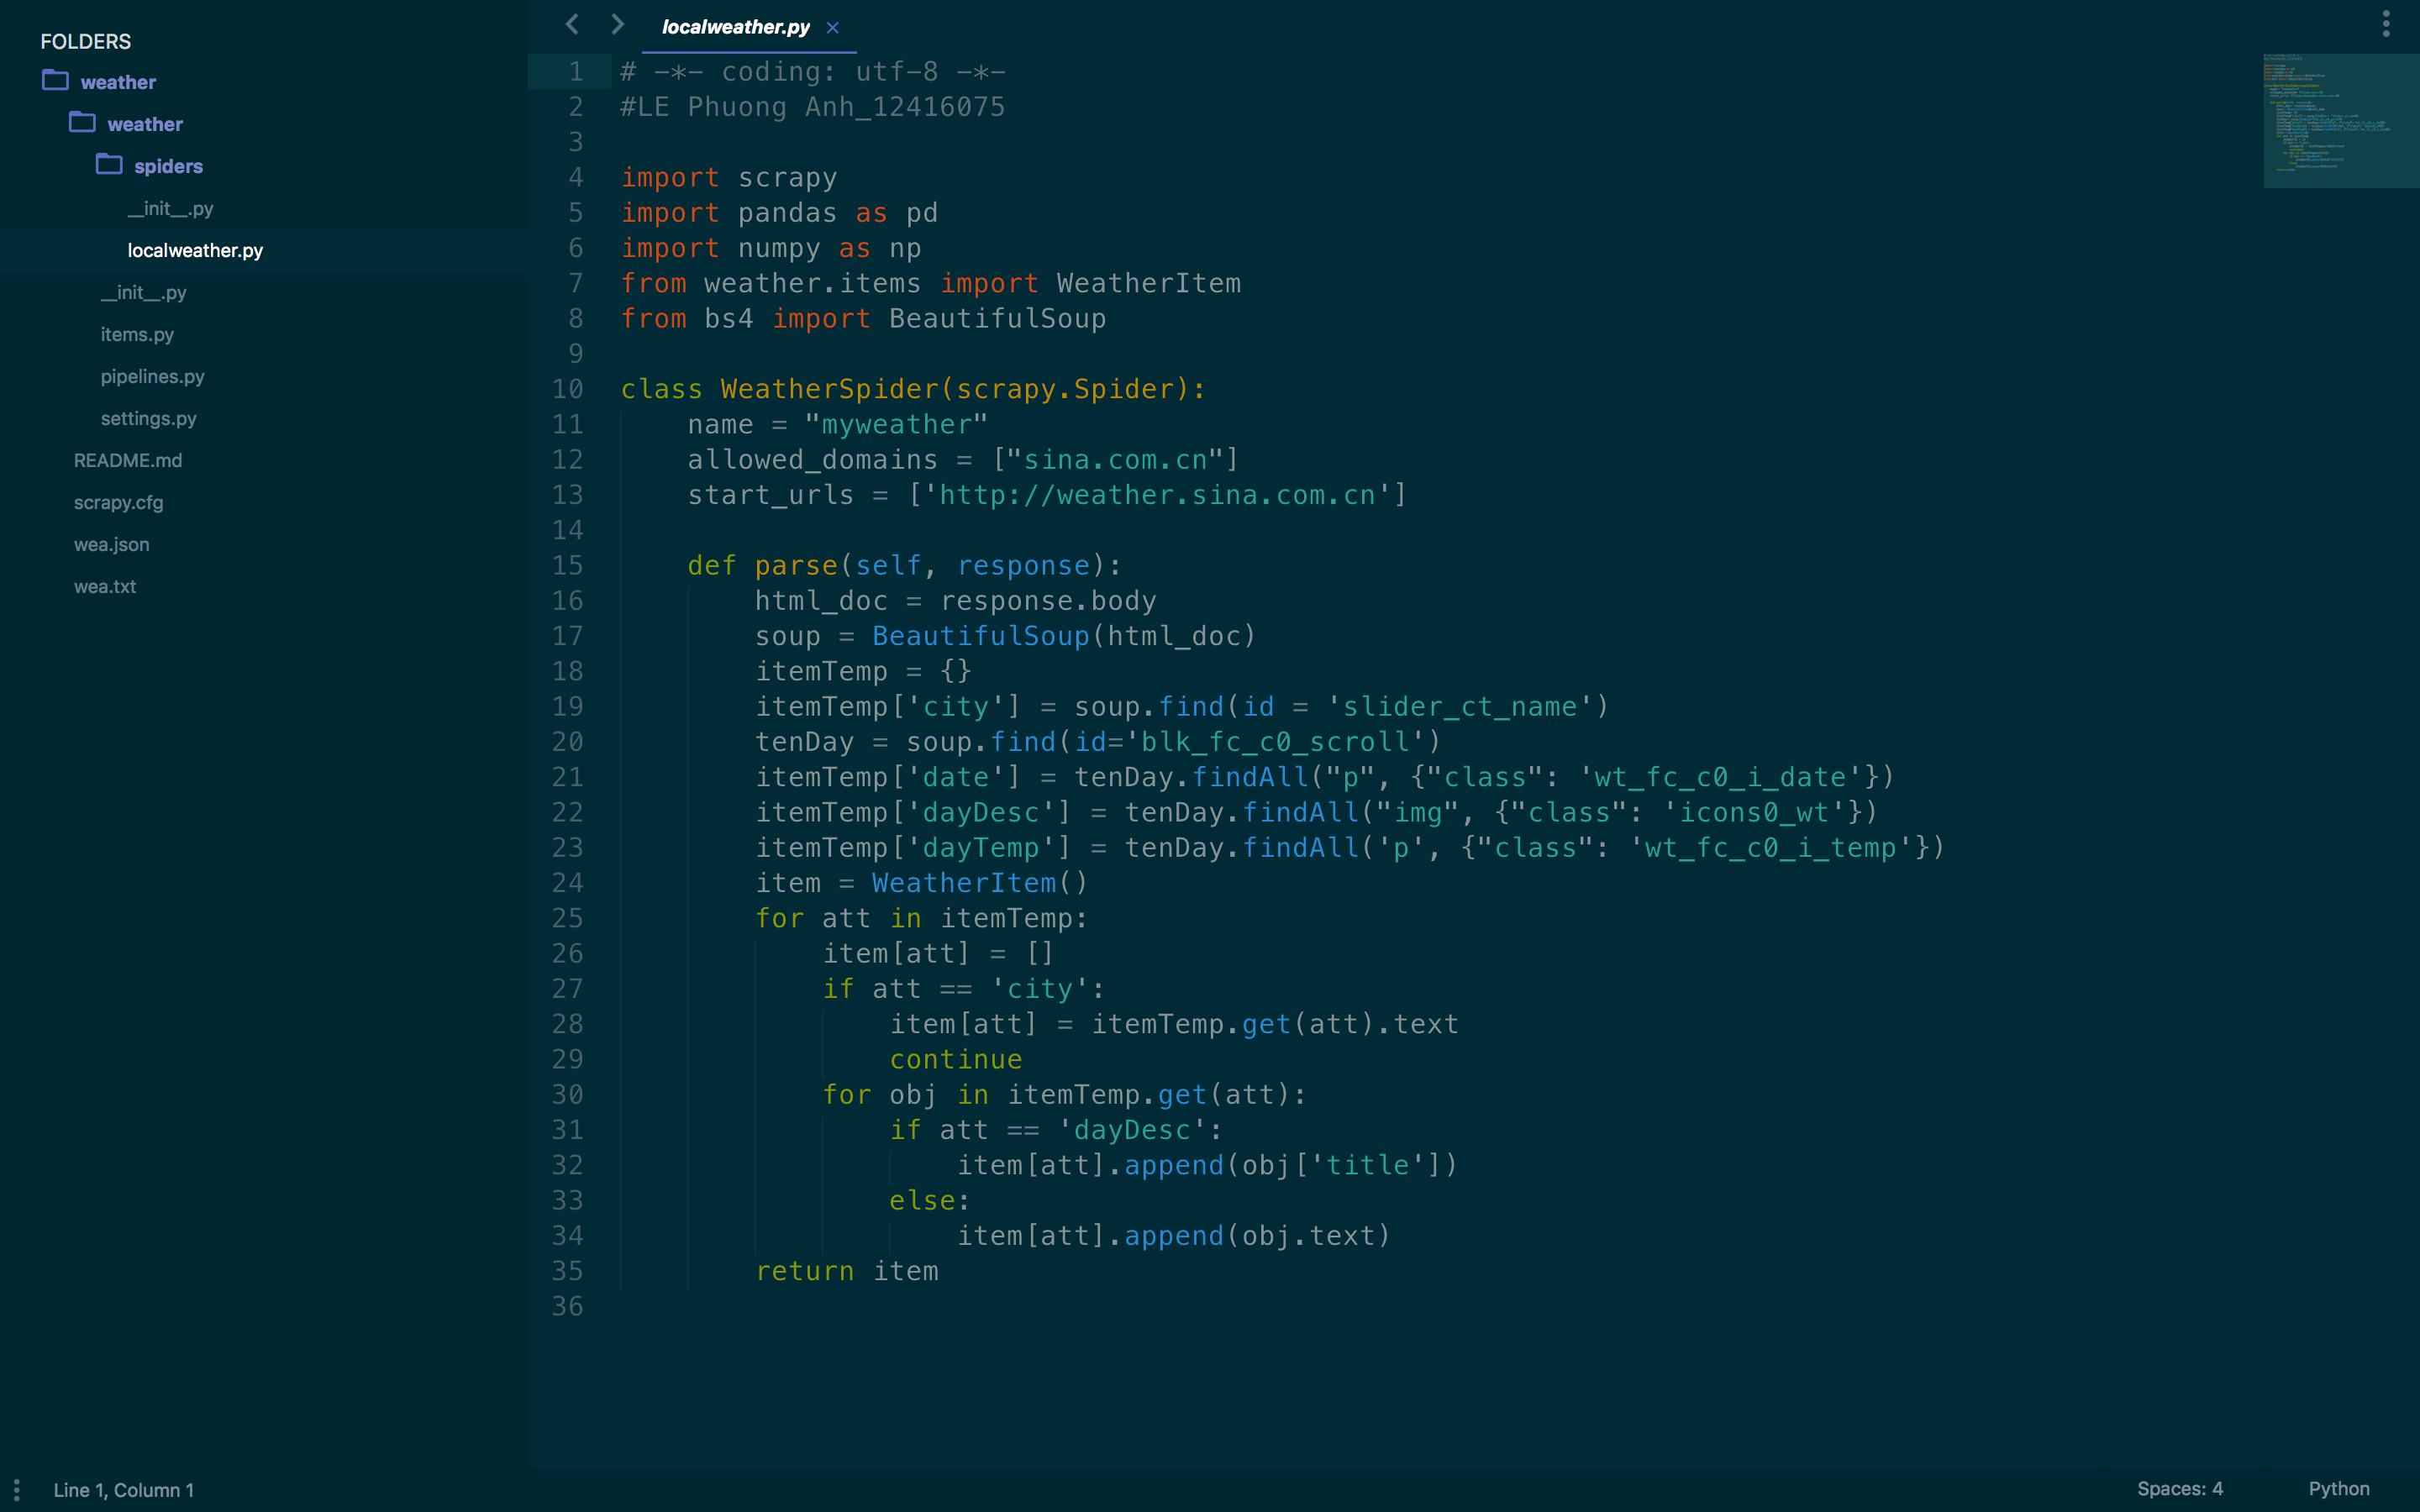
\includegraphics[width=\linewidth]{main}
  \caption{Main program.}
  \label{fig:MainCode}
 \end{center}
\end{figure}
\begin{figure}[h]
  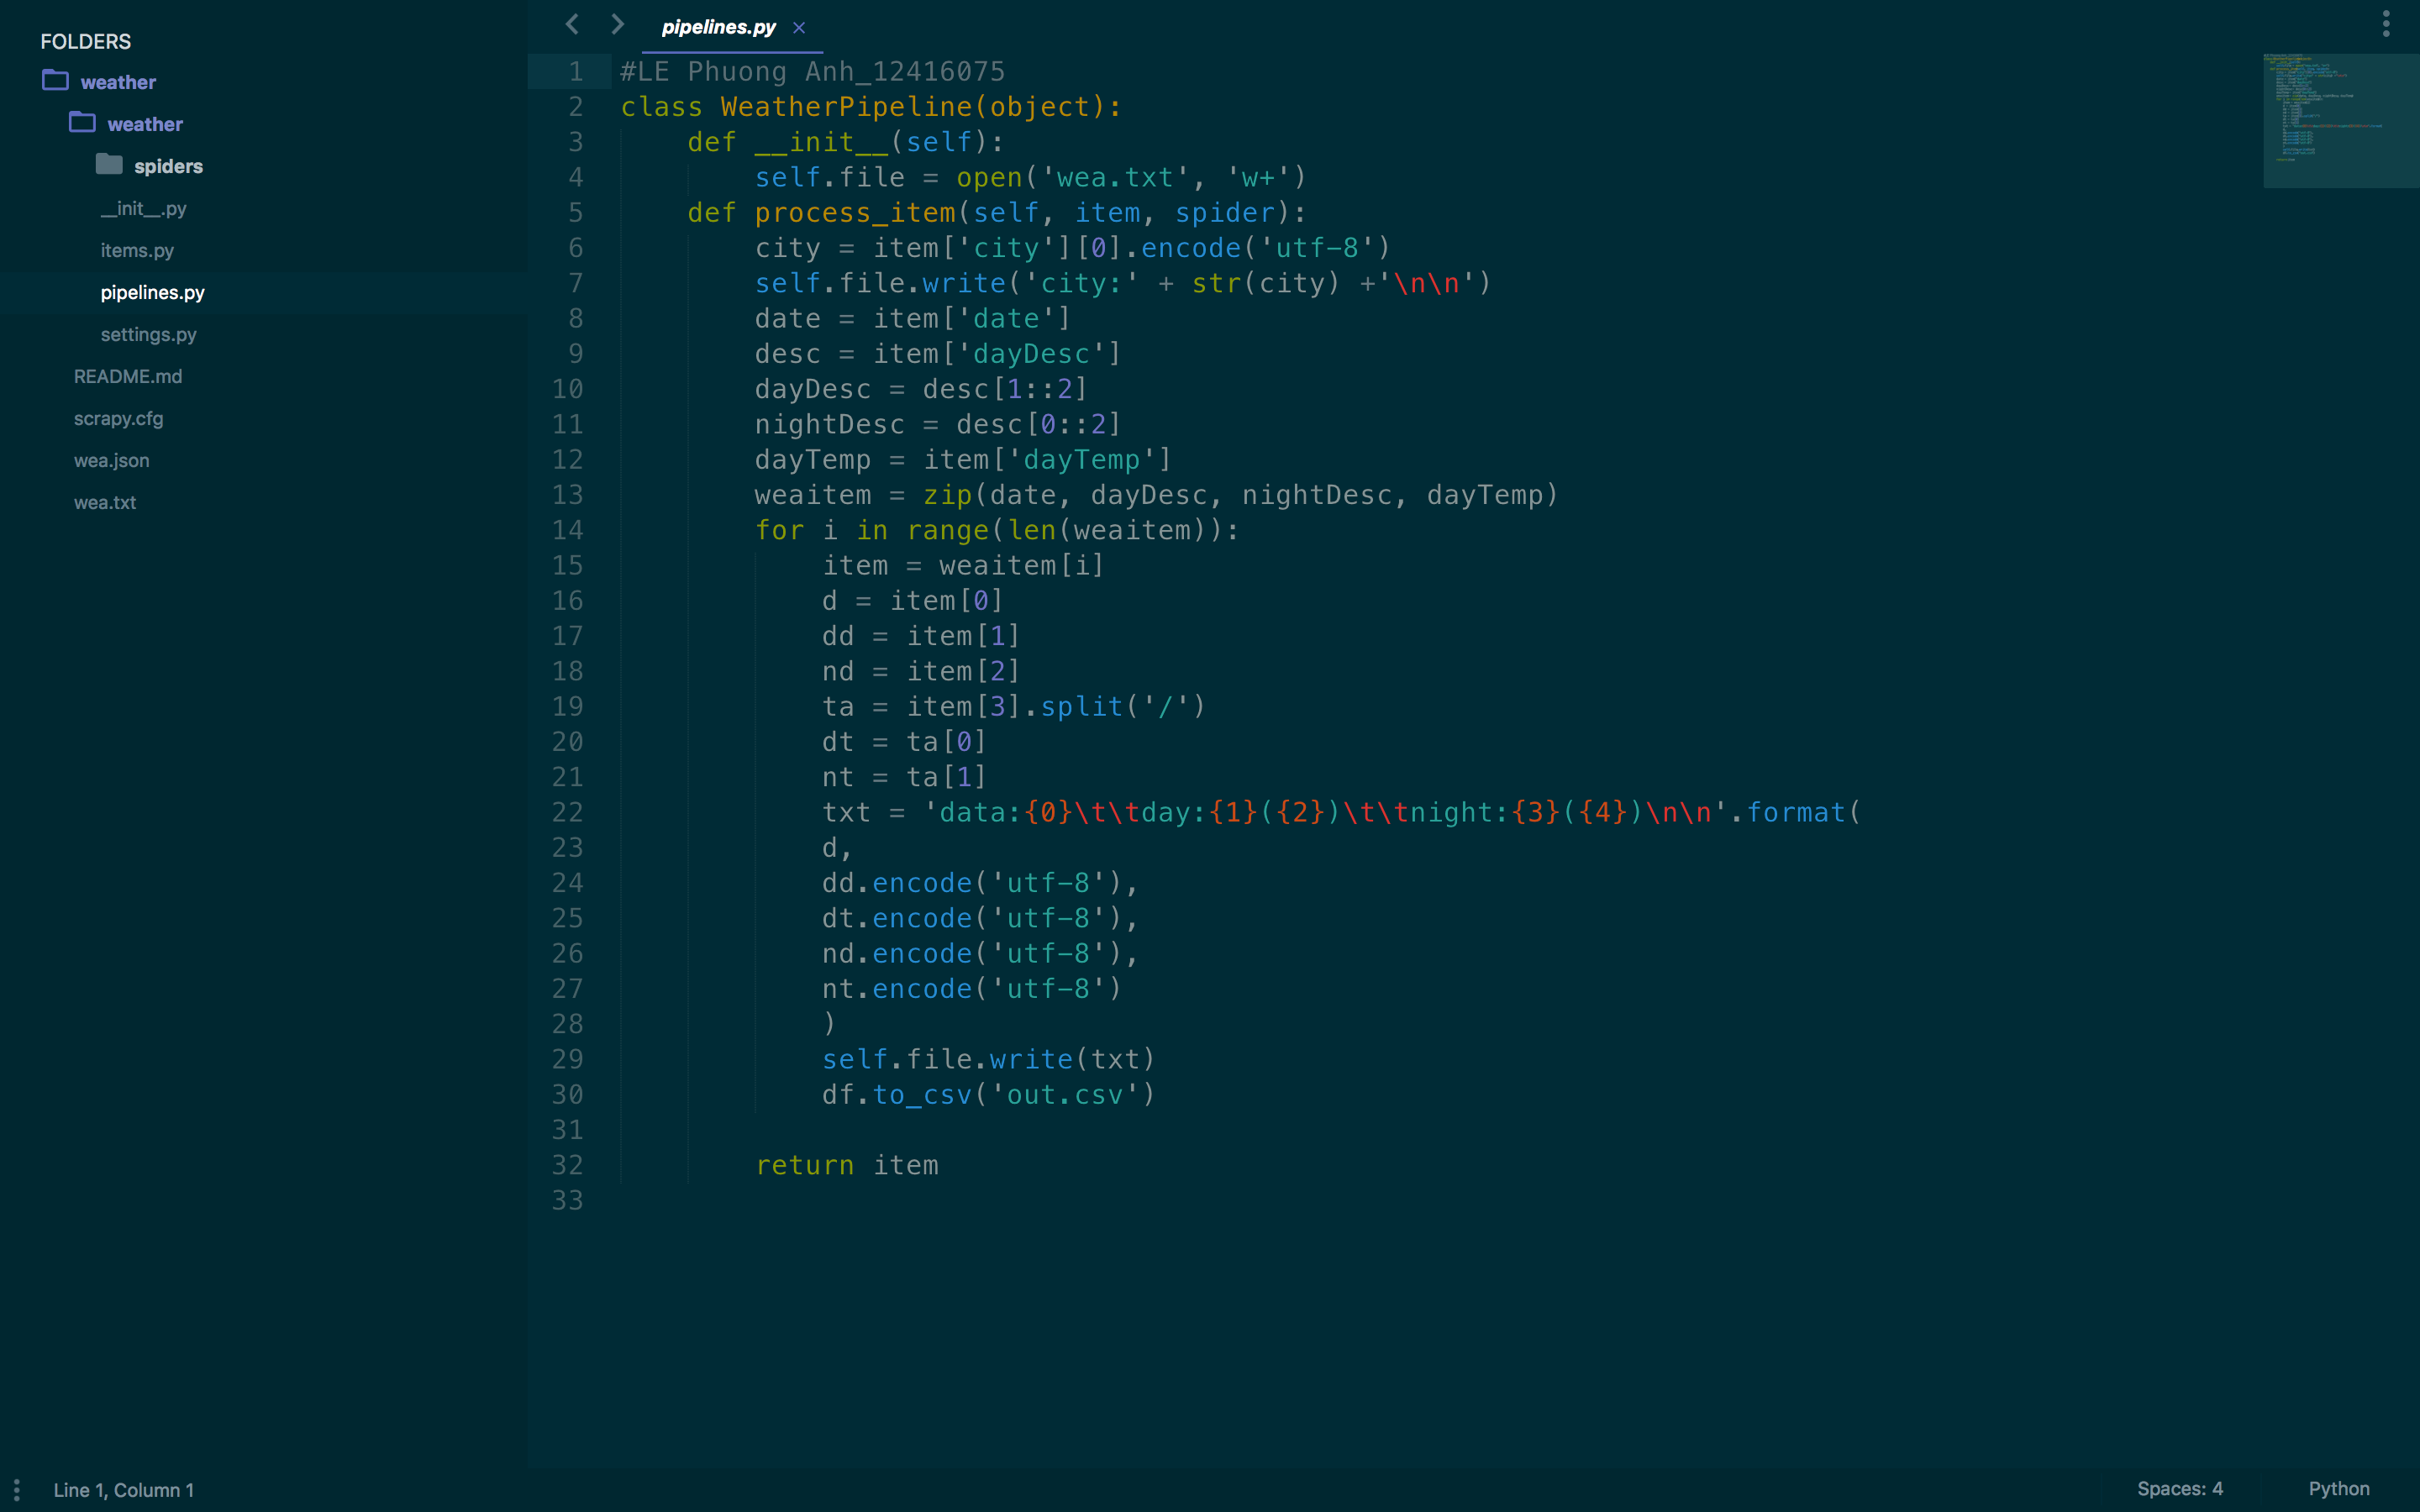
\includegraphics[width=\linewidth]{item1}
  \caption{Weather Pipe Line}
  \label{fig:WeatherPLine}
\end{figure}
\begin{figure}[ht]
  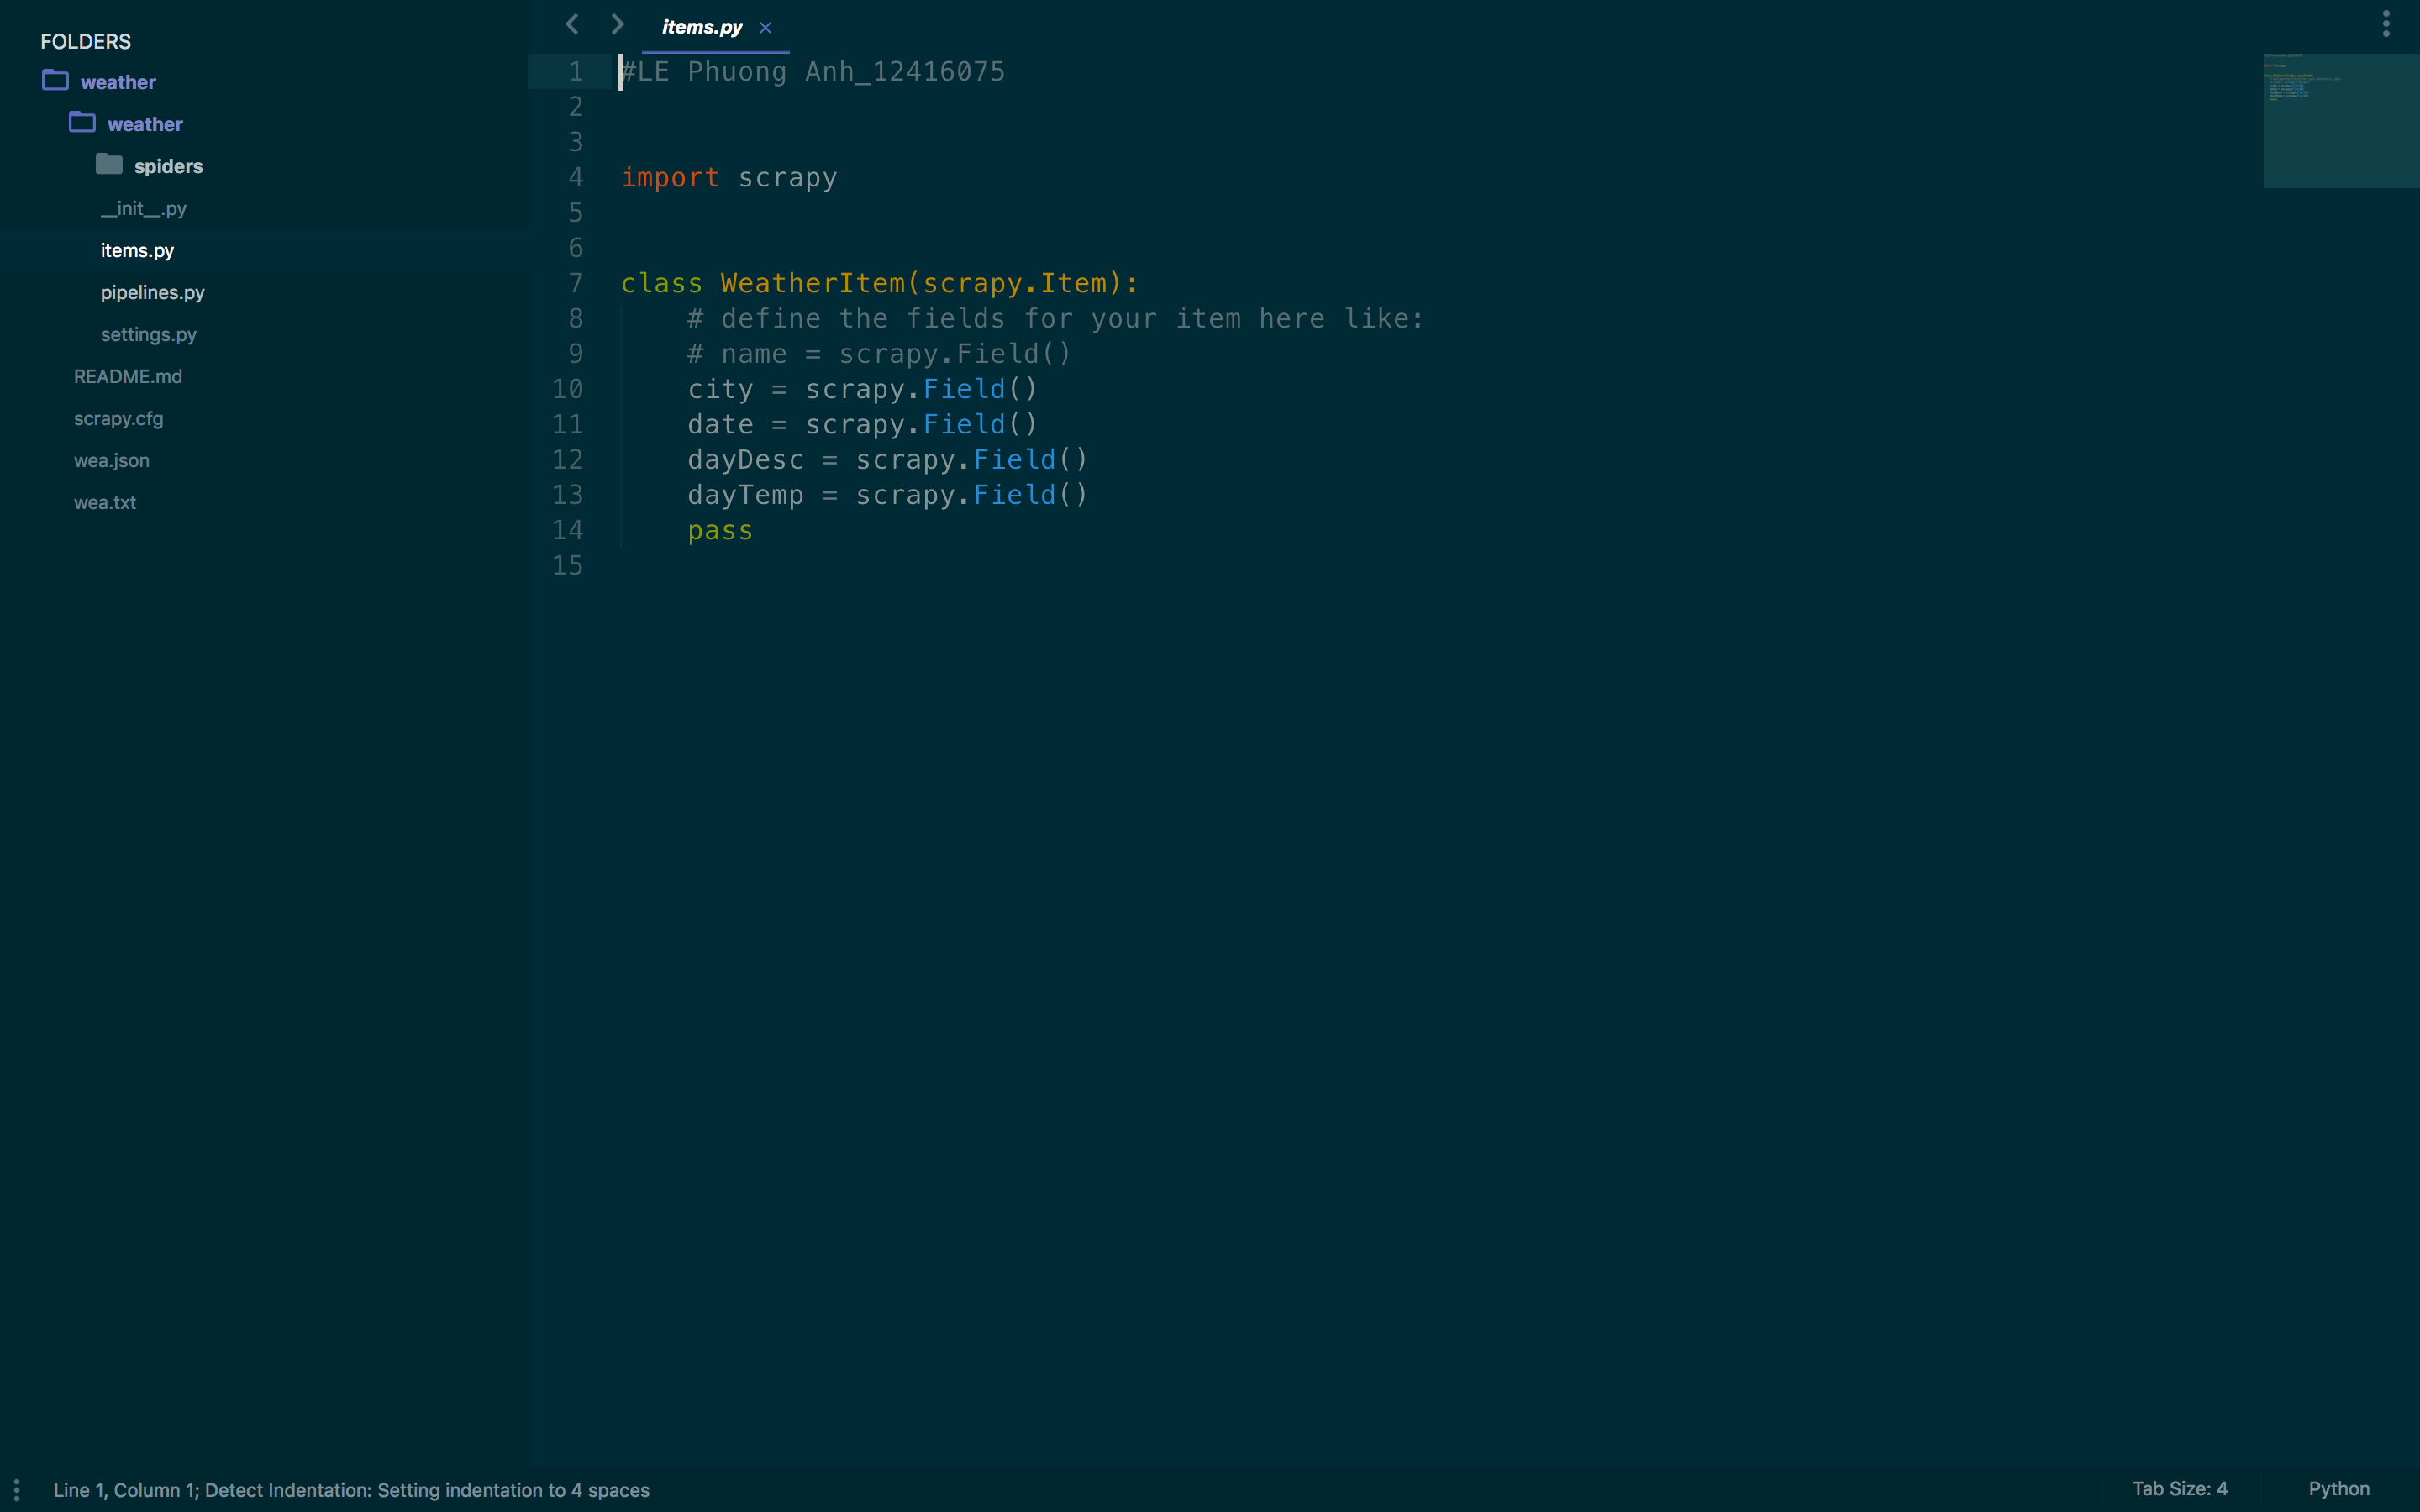
\includegraphics[width=\linewidth]{item2}
  \caption{Weather Item}
  \label{fig:WeatherItem}
\end{figure}
\begin{figure}[ht]
  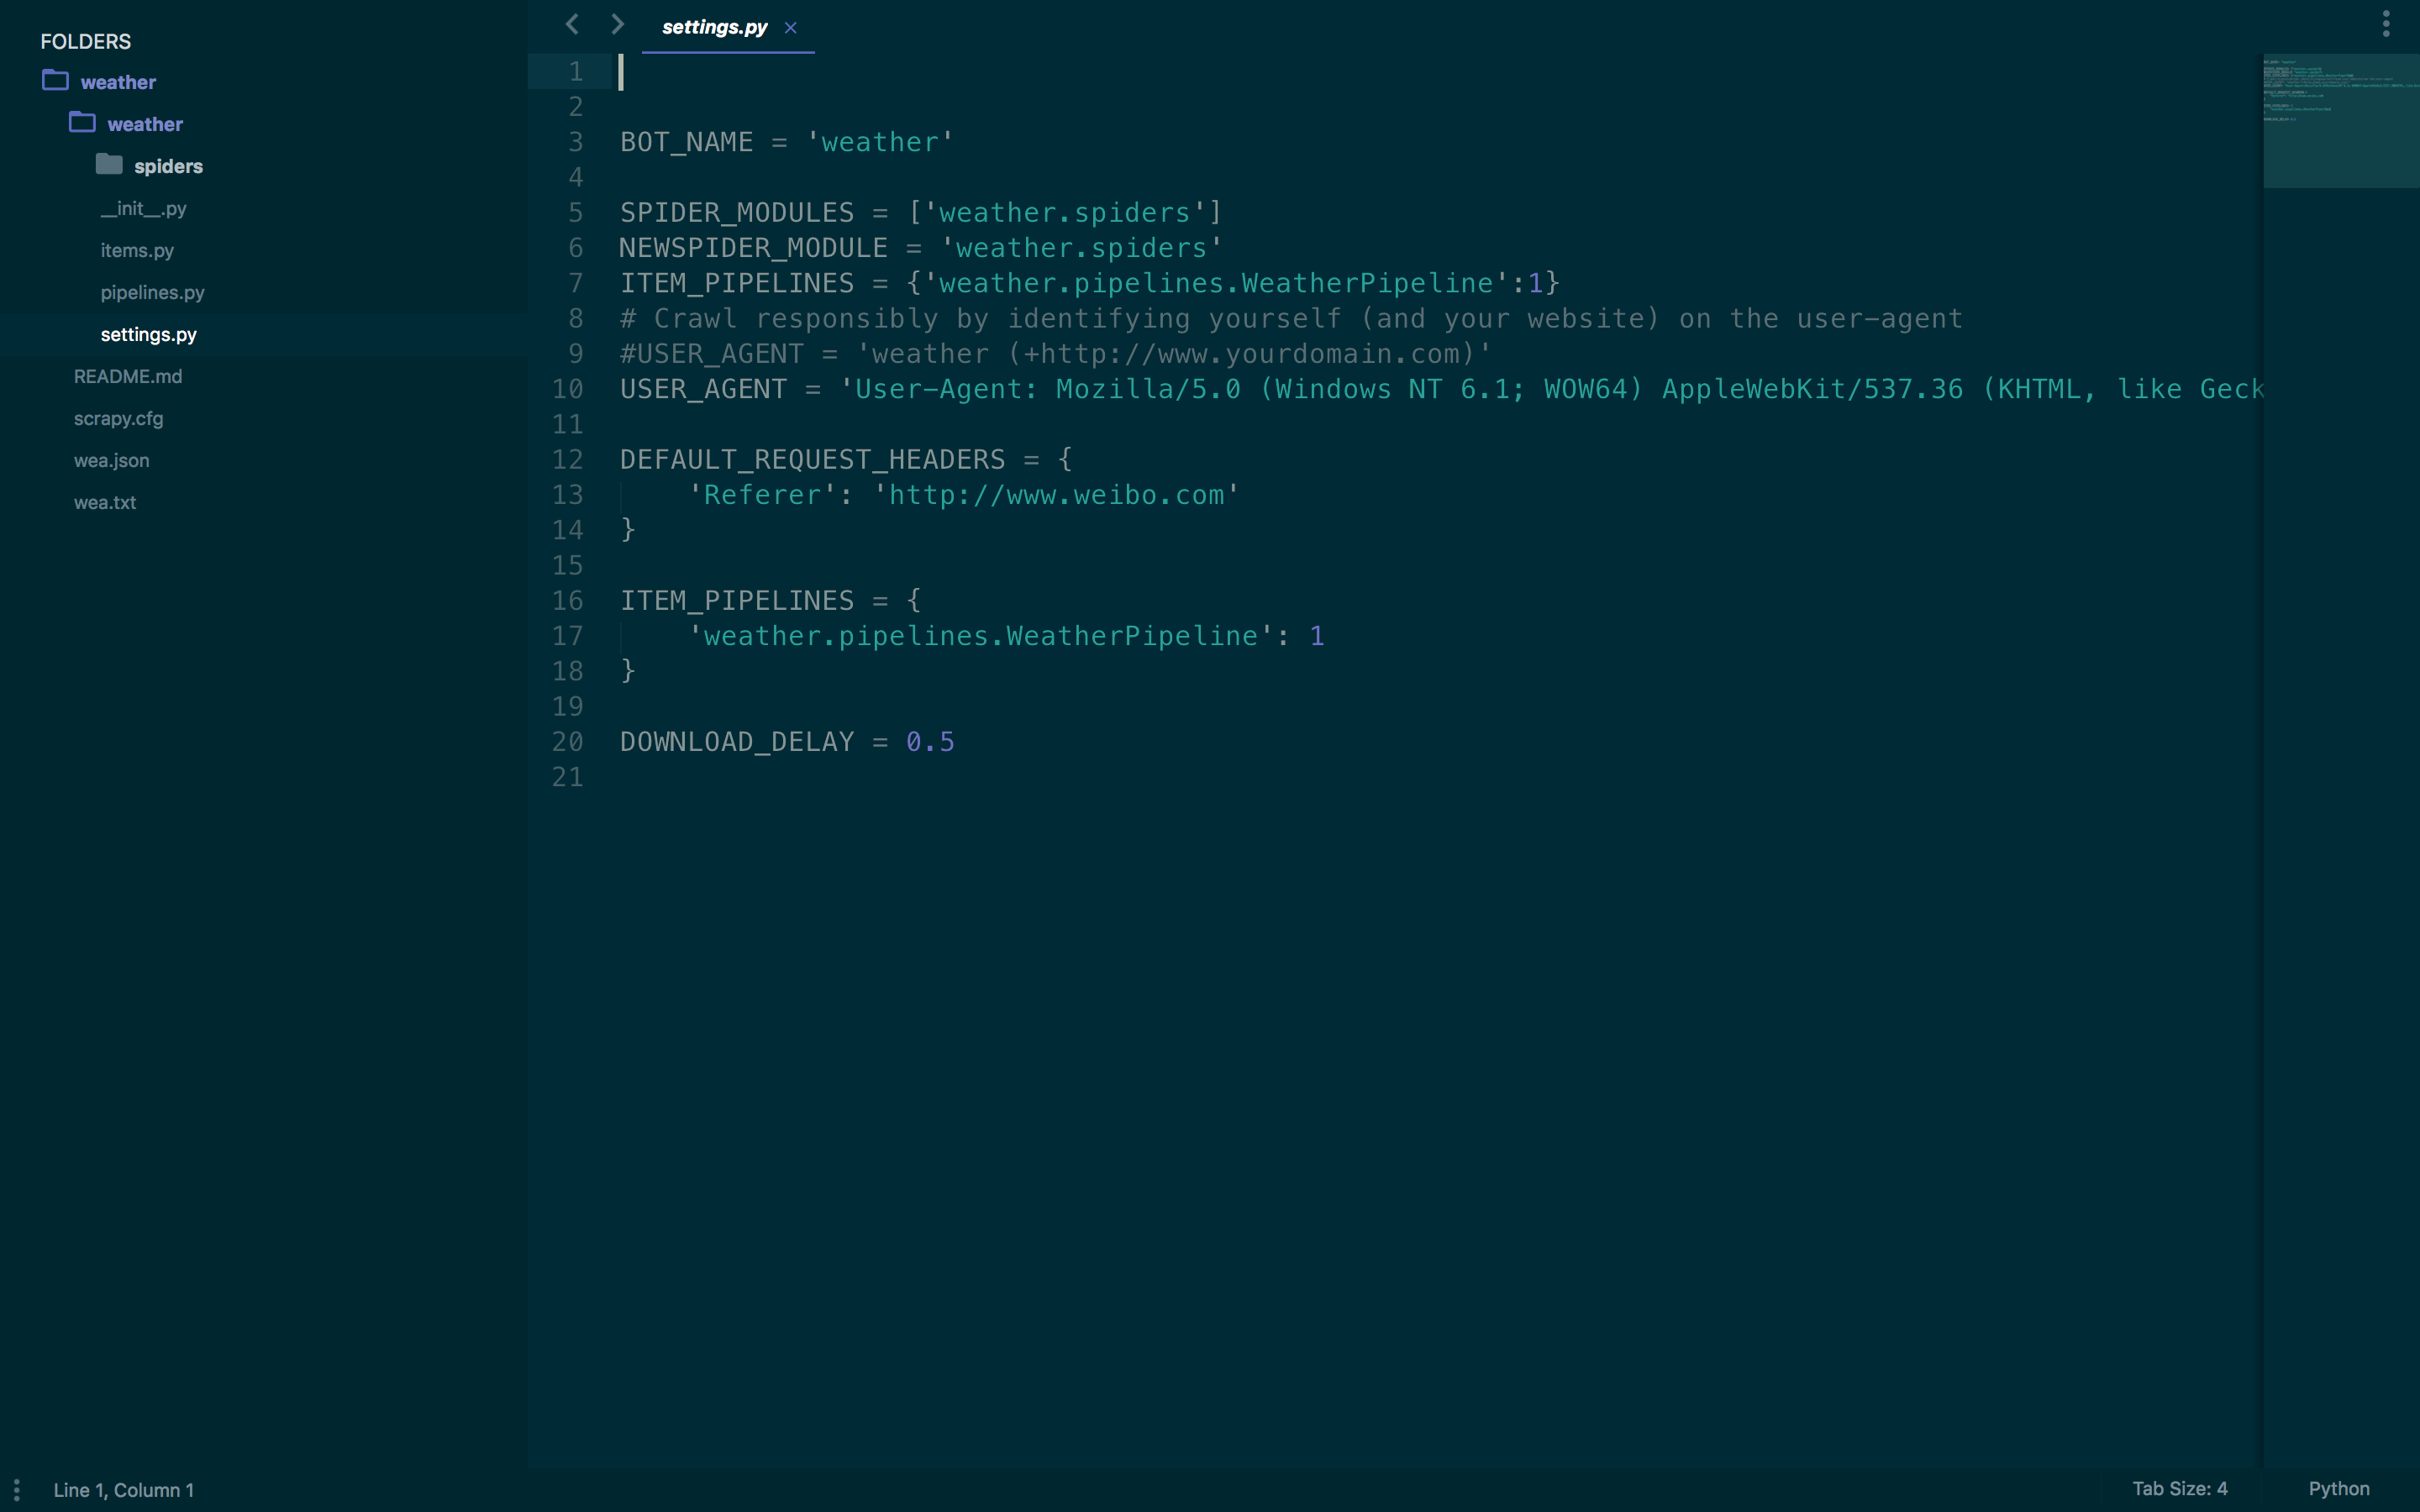
\includegraphics[width=\linewidth]{item3}
  \caption{Setting}
  \label{fig:Setting}
\end{figure}
\begin{figure}[ht]
  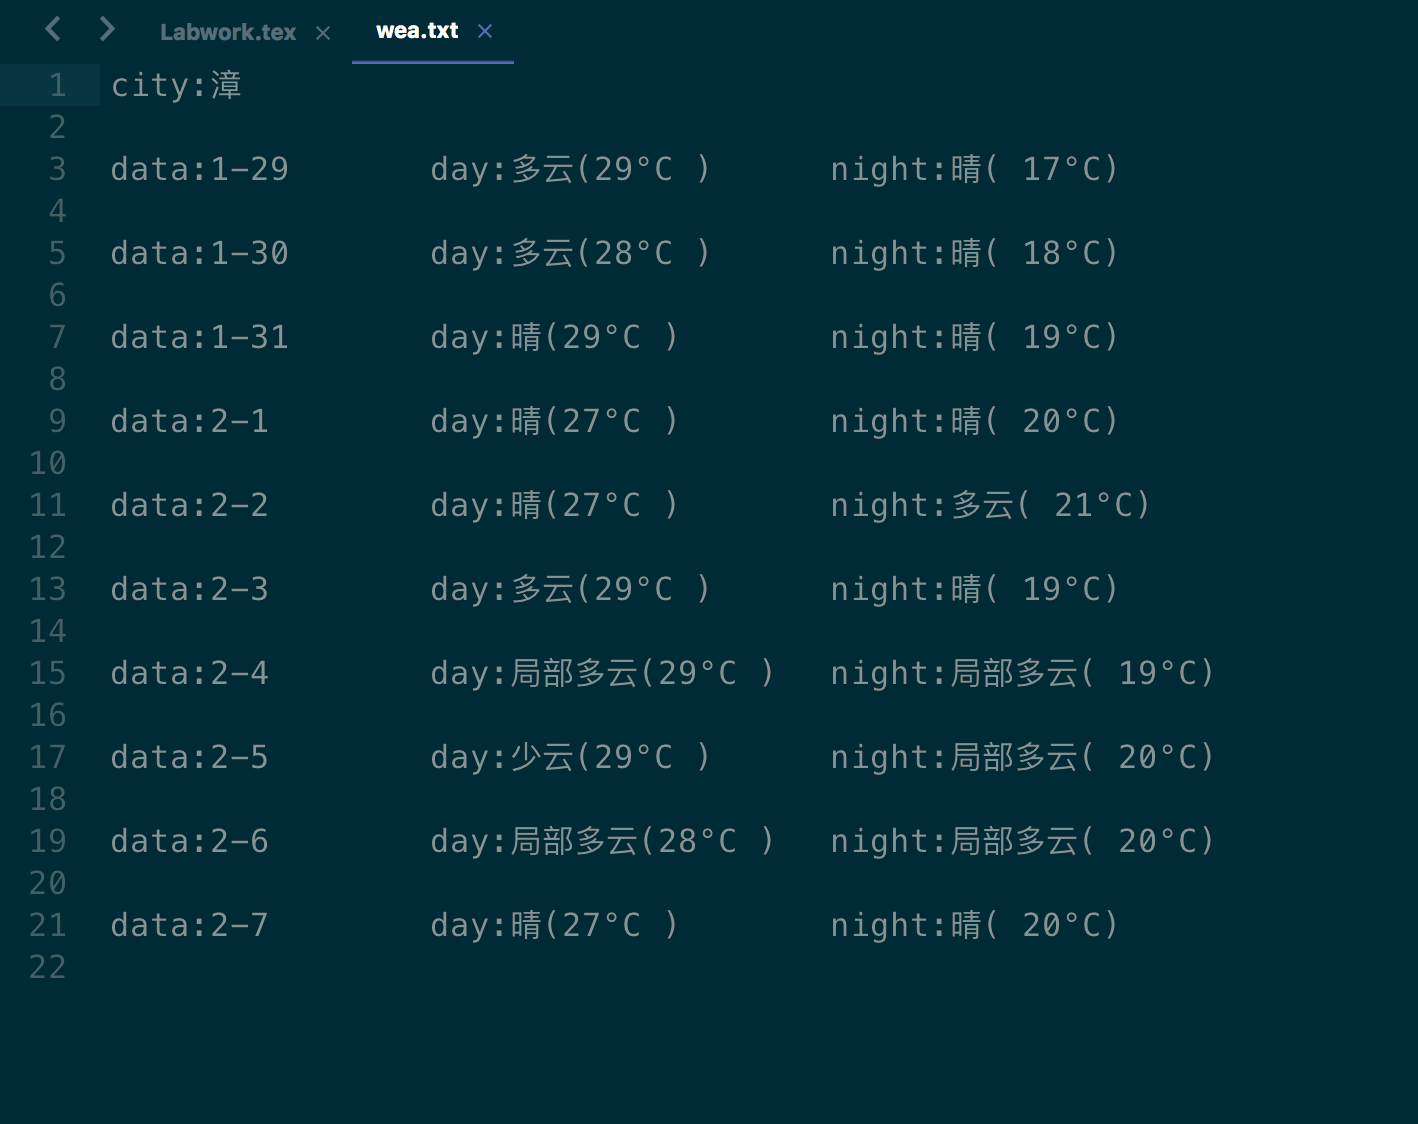
\includegraphics[width=\linewidth]{item4}
  \caption{Output}
  \label{fig:Output}
\end{figure}
\end{document}
